\documentclass{standalone}

\usepackage[dvipsnames]{xcolor}
\usepackage{tikz}

\begin{document}

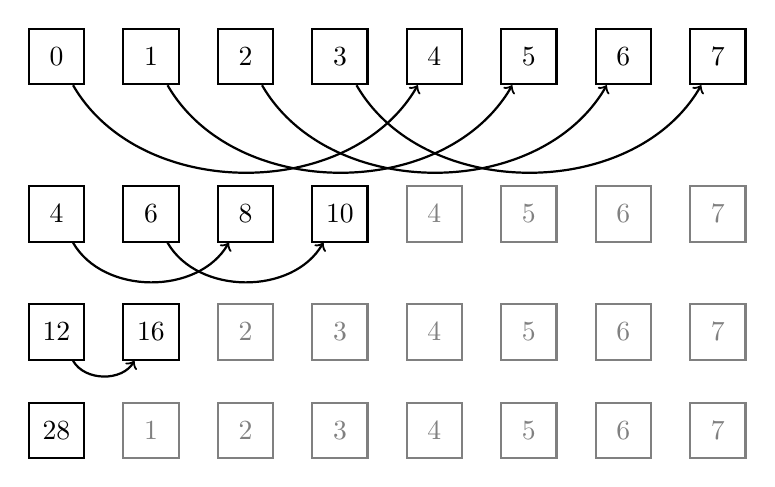
\begin{tikzpicture}[thick]
  \tikzset{box/.style={draw, rectangle, inner sep=10pt}}

  \foreach \i in {0, 1, ..., 7} {
    \path ({\i * 1.2}, 0) coordinate [box] (0-\i) node {\i};
  }

  \draw [->] (0-0) to [out=300, in=240] (0-4);
  \draw [->] (0-1) to [out=300, in=240] (0-5);
  \draw [->] (0-2) to [out=300, in=240] (0-6);
  \draw [->] (0-3) to [out=300, in=240] (0-7);

  \foreach \i/\v in {0/4, 1/6, 2/8, 3/10} {
      \path ({\i * 1.2}, -2) coordinate [box] (1-\i) node {\v};
  }
  \foreach \i in {4, 5, 6, 7} {
    \path ({\i * 1.2}, -2)
          coordinate [box, Gray] (1-\i) node {\color{gray}\i};
  }

  \draw [->] (1-0) to [out=300, in=240] (1-2);
  \draw [->] (1-1) to [out=300, in=240] (1-3);

  \foreach \i/\v in {0/12, 1/16} {
      \path ({\i * 1.2}, -3.5) coordinate [box] (2-\i) node {\v};
  }
  \foreach \i in {2, ..., 7} {
    \path ({\i * 1.2}, -3.5)
          coordinate [box, Gray] (2-\i) node {\color{gray}\i};
  }

  \draw [->] (2-0) to [out=300, in=240] (2-1);

  \path (0, -4.75) coordinate [box] (3-0) node {28};
  \foreach \i in {1, ..., 7} {
    \path ({\i * 1.2}, -4.75)
          coordinate [box, Gray] (3-\i) node {\color{gray}\i};
  }


\end{tikzpicture}

\end{document}
